\documentclass[aspectratio=43]{beamer}

% Text packages to stop warnings
\usepackage{lmodern}
\usepackage{textcomp}
\usepackage{ulem}
\usepackage[utf8]{inputenc}
\usepackage[T1]{fontenc}

\usepackage{listings}
\usepackage{tikz}
\usetikzlibrary{arrows,decorations.pathreplacing,positioning}

% Themes
\usetheme{Boadilla}
\setbeamertemplate{footline}[page number]{}
\setbeamertemplate{navigation symbols}{}

% Suppress the navigation bar
\beamertemplatenavigationsymbolsempty

\newenvironment{changemargin}[1]{% 
  \begin{list}{}{% 
    \setlength{\topsep}{0pt}% 
    \setlength{\leftmargin}{#1}% 
    \setlength{\rightmargin}{1em}
    \setlength{\listparindent}{\parindent}% 
    \setlength{\itemindent}{\parindent}% 
    \setlength{\parsep}{\parskip}% 
  }% 
  \item[]}{\end{list}} 

\lstset{basicstyle=\scriptsize, frame=single}

\lstdefinelanguage{JavaScript}{
  keywords={typeof, new, true, false, catch, function, return, null, catch, switch, var, if, in, while, do, else, case, break},
  keywordstyle=\color{blue}\bfseries,
  ndkeywords={class, export, boolean, throw, implements, import, this},
  ndkeywordstyle=\color{darkgray}\bfseries,
  identifierstyle=\color{black},
  sensitive=false,
  comment=[l]{//},
  morecomment=[s]{/*}{*/},
  commentstyle=\color{purple}\ttfamily,
  stringstyle=\color{red}\ttfamily,
  morestring=[b]',
  morestring=[b]"
}

\title{Lecture 26---More Profiling: gperftools, \\ systemwide tools: oprofile, perf, DTrace, etc.}
\subtitle{ECE 459: Programming for Performance}
\date{March 11, 2015}

\begin{document}
%%%%%%%%%%%%%%%%%%%%%%%%%%%%%%%%%%%%%%%%%%%%%%%%%%%%%%%%%%%%%%%%%%%%%%%%%%%%%%%%
\begin{frame}[plain]
  \titlepage
\end{frame}
%%%%%%%%%%%%%%%%%%%%%%%%%%%%%%%%%%%%%%%%%%%%%%%%%%%%%%%%%%%%%%%%%%%%%%%%%%%%%%%%

\part{gperftools}
\frame{\partpage}

%%%%%%%%%%%%%%%%%%%%%%%%%%%%%%%%%%%%%%%%%%%%%%%%%%%%%%%%%%%%%%%%%%%%%%%%%%%%%%%%
\begin{frame}
  \frametitle{Introduction to gperftools}

  \begin{changemargin}{2cm}
    Google Performance Tools include:
      
      \begin{itemize}
        \item CPU profiler.
        \item Heap profiler.
        \item Heap checker.
        \item Faster (multithreaded) {\tt malloc}.
      \end{itemize}
~\\[1em]
     We'll mostly use the CPU profiler:
      \begin{itemize}
        \item purely statistical sampling;
        \item no recompilation; at most linking; and
        \item built-in visual output.
      \end{itemize}
  \end{changemargin}
\end{frame}
%%%%%%%%%%%%%%%%%%%%%%%%%%%%%%%%%%%%%%%%%%%%%%%%%%%%%%%%%%%%%%%%%%%%%%%%%%%%%%%%

%%%%%%%%%%%%%%%%%%%%%%%%%%%%%%%%%%%%%%%%%%%%%%%%%%%%%%%%%%%%%%%%%%%%%%%%%%%%%%%%
\begin{frame}[fragile]
  \frametitle{Google Perf Tools profiler usage}

  \begin{changemargin}{2cm}
    You can use the profiler without any recompilation.
      \begin{itemize}
        \item Not recommended---worse data.
      \end{itemize}

  \begin{lstlisting}
LD_PRELOAD="/usr/lib/libprofiler.so" \
CPUPROFILE=test.prof ./test
  \end{lstlisting}

     The other option is to link to the profiler:
      \begin{itemize}
        \item {\tt -lprofiler}
      \end{itemize}
    Both options read the {\tt CPUPROFILE} environment variable:
      \begin{itemize}
        \item states the location to write the profile data.
      \end{itemize}
  \end{changemargin}
\end{frame}
%%%%%%%%%%%%%%%%%%%%%%%%%%%%%%%%%%%%%%%%%%%%%%%%%%%%%%%%%%%%%%%%%%%%%%%%%%%%%%%%

%%%%%%%%%%%%%%%%%%%%%%%%%%%%%%%%%%%%%%%%%%%%%%%%%%%%%%%%%%%%%%%%%%%%%%%%%%%%%%%%
\begin{frame}[fragile]
  \frametitle{Other Usage}

  \begin{changemargin}{2cm}
     You can use the profiling library directly as well:
      \begin{itemize}
        \item {\tt \#include <gperftools/profiler.h>}
      \end{itemize}
     Bracket code you want profiled with:
      \begin{itemize}
        \item {\tt ProfilerStart()}
        \item {\tt ProfilerEnd()}
      \end{itemize}~\\
    
    You can change the sampling frequency with the
      {\tt CPUPROFILE\_FREQUENCY} environment variable.
      \begin{itemize}
        \item {\bf Default value:} 100
      \end{itemize}
  \end{changemargin}
\end{frame}
%%%%%%%%%%%%%%%%%%%%%%%%%%%%%%%%%%%%%%%%%%%%%%%%%%%%%%%%%%%%%%%%%%%%%%%%%%%%%%%%

%%%%%%%%%%%%%%%%%%%%%%%%%%%%%%%%%%%%%%%%%%%%%%%%%%%%%%%%%%%%%%%%%%%%%%%%%%%%%%%%
\begin{frame}[fragile]
  \frametitle{{\tt pprof} Usage}

  \begin{changemargin}{1.5cm}
    Like {\tt gprof}, it will analyze profiling results.

  \begin{lstlisting}
% pprof test test.prof
    Enters "interactive" mode
% pprof --text test test.prof
    Outputs one line per procedure
% pprof --gv test test.prof
     Displays annotated call-graph via 'gv'
% pprof --gv --focus=Mutex test test.prof
    Restricts to code paths including a .*Mutex.* entry
% pprof --gv --focus=Mutex --ignore=string test test.prof
    Code paths including Mutex but not string
% pprof --list=getdir test test.prof
    (Per-line) annotated source listing for getdir()
% pprof --disasm=getdir test test.prof
    (Per-PC) annotated disassembly for getdir()
  \end{lstlisting}

    Can also output {\tt dot}, {\tt ps}, {\tt pdf} or {\tt gif} instead of
      {\tt gv}.
  \end{changemargin}

\end{frame}
%%%%%%%%%%%%%%%%%%%%%%%%%%%%%%%%%%%%%%%%%%%%%%%%%%%%%%%%%%%%%%%%%%%%%%%%%%%%%%%%

%%%%%%%%%%%%%%%%%%%%%%%%%%%%%%%%%%%%%%%%%%%%%%%%%%%%%%%%%%%%%%%%%%%%%%%%%%%%%%%%
\begin{frame}[fragile]
  \frametitle{Text Output}

  \begin{changemargin}{1.5cm}
    Similar to the flat profile in {\tt gprof}

  \begin{lstlisting}
jon@riker examples master % pprof --text test test.prof 
Using local file test.
Using local file test.prof.
Removing killpg from all stack traces.
Total: 300 samples
      95  31.7%  31.7%      102  34.0% int_power
      58  19.3%  51.0%       58  19.3% float_power
      51  17.0%  68.0%       96  32.0% float_math_helper
      50  16.7%  84.7%      137  45.7% int_math_helper
      18   6.0%  90.7%      131  43.7% float_math
      14   4.7%  95.3%      159  53.0% int_math
      14   4.7% 100.0%      300 100.0% main
       0   0.0% 100.0%      300 100.0% __libc_start_main
       0   0.0% 100.0%      300 100.0% _start
  \end{lstlisting}
  \end{changemargin}

\end{frame}
%%%%%%%%%%%%%%%%%%%%%%%%%%%%%%%%%%%%%%%%%%%%%%%%%%%%%%%%%%%%%%%%%%%%%%%%%%%%%%%%

%%%%%%%%%%%%%%%%%%%%%%%%%%%%%%%%%%%%%%%%%%%%%%%%%%%%%%%%%%%%%%%%%%%%%%%%%%%%%%%%
\begin{frame}
  \frametitle{Text Output Explained}

  \begin{changemargin}{2cm}
    Columns, from left to right:\\[1em]

    Number of checks (samples) in this function.\\
    Percentage of checks in this function.
      \begin{itemize}
        \item Same as {\bf time} in {\tt gprof}.\\[1em]
      \end{itemize}
    Percentage of checks in the functions printed so far.
      \begin{itemize}
        \item Equivalent to {\bf cumulative} (but in \%).\\[1em]
      \end{itemize}
    Number of checks in this function and its callees.\\
    Percentage of checks in this function and its callees.\\
    Function name.
  \end{changemargin}
\end{frame}
%%%%%%%%%%%%%%%%%%%%%%%%%%%%%%%%%%%%%%%%%%%%%%%%%%%%%%%%%%%%%%%%%%%%%%%%%%%%%%%%

%%%%%%%%%%%%%%%%%%%%%%%%%%%%%%%%%%%%%%%%%%%%%%%%%%%%%%%%%%%%%%%%%%%%%%%%%%%%%%%%
\begin{frame}
  \frametitle{Graphical Output}

  \begin{center}
    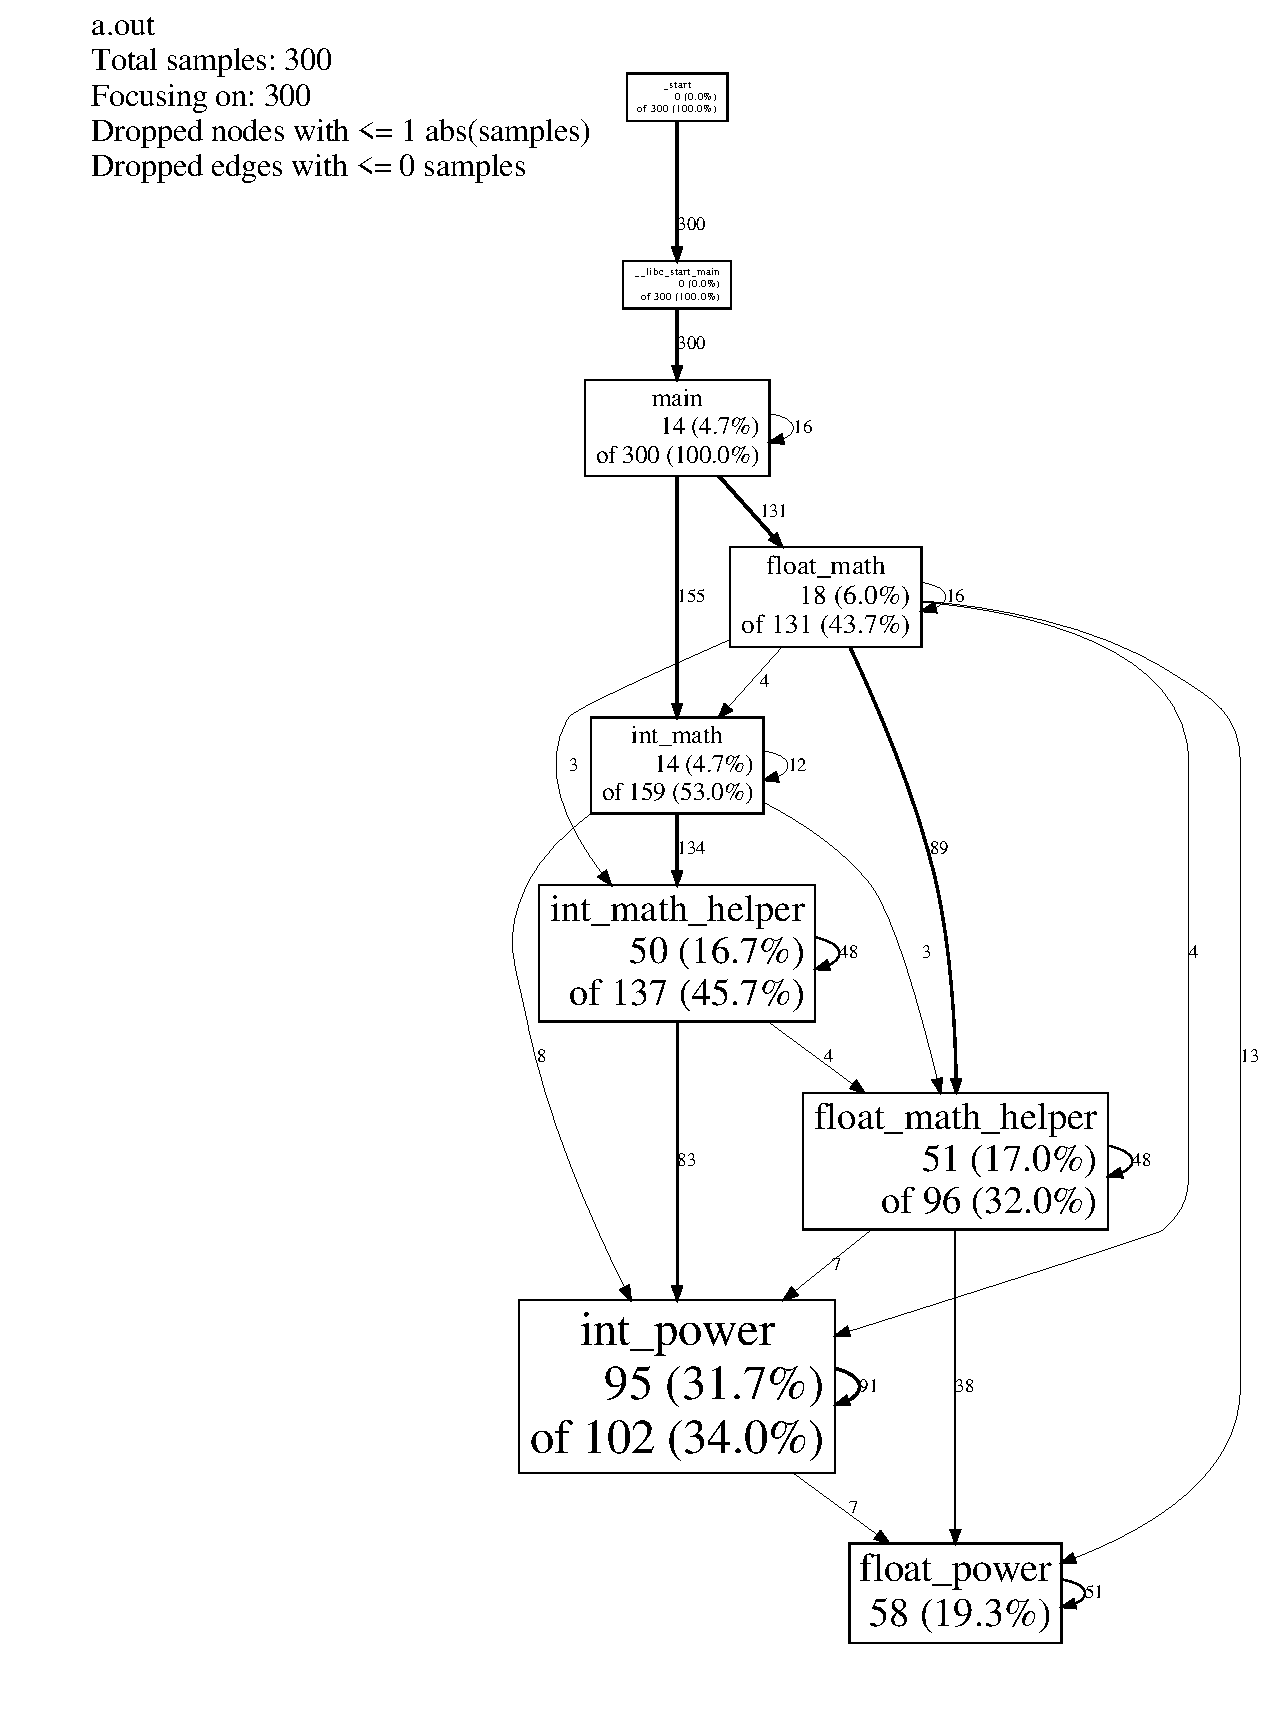
\includegraphics[scale=0.25]{L26/test}
  \end{center}
\end{frame}
%%%%%%%%%%%%%%%%%%%%%%%%%%%%%%%%%%%%%%%%%%%%%%%%%%%%%%%%%%%%%%%%%%%%%%%%%%%%%%%%

%%%%%%%%%%%%%%%%%%%%%%%%%%%%%%%%%%%%%%%%%%%%%%%%%%%%%%%%%%%%%%%%%%%%%%%%%%%%%%%%
\begin{frame}
  \frametitle{Graphical Output Explained}

  \begin{changemargin}{2cm}
  Output was too small to read on the slide.

  \begin{itemize}
    \item Shows the same numbers as the text output.
    \item Directed edges denote function calls.
    \item Note: number of samples in callees = \\
      \qquad number in ``this function + callees'' - \\
      \qquad number in ``this function''.\\
    \item {\bf Example:}\\
{{\tt float\_math\_helper}, 51 (local) of 96 (cumulative)} \\
      96 - 51 = 45 (callees)
      \begin{itemize}
        \item callee {\tt int\_power} = 7 (bogus)
        \item callee {\tt float\_power} = 38
        \item callees total = 45
      \end{itemize}

  \end{itemize}
  \end{changemargin}
\end{frame}
%%%%%%%%%%%%%%%%%%%%%%%%%%%%%%%%%%%%%%%%%%%%%%%%%%%%%%%%%%%%%%%%%%%%%%%%%%%%%%%%

%%%%%%%%%%%%%%%%%%%%%%%%%%%%%%%%%%%%%%%%%%%%%%%%%%%%%%%%%%%%%%%%%%%%%%%%%%%%%%%%
\begin{frame}
  \frametitle{Things You May Notice}

  \begin{changemargin}{2cm}
    Call graph is not exact.
    
      \begin{itemize}
        \item In fact, it shows many bogus relations which clearly don't exist.
        \item For instance, we know that there are no cross-calls between {\tt int} and {\tt float} functions.
      \end{itemize}~\\

    As with {\tt gprof}, optimizations will change the
      graph.\\[1em]

    You'll probably want to look at the text profile first, then use the
      {\tt --focus} flag to look at individual functions.
  \end{changemargin}
\end{frame}
%%%%%%%%%%%%%%%%%%%%%%%%%%%%%%%%%%%%%%%%%%%%%%%%%%%%%%%%%%%%%%%%%%%%%%%%%%%%%%%%

% How to Read
% http://www.cs.utah.edu/dept/old/texinfo/as/gprof.html
% http://www.civilnet.cn/book/kernel/GNU.Linux.Application.Programming/LiB0055.html
% http://ececmpsysweb.groups.et.byu.net/cmpsys.2004.winter/citizenship/Bryan_Wheeler/Profiling_Tutorial.html

% gprof
% OProfile
% Valgrind
% Intel VTune
% AMD CodeAnalyst

\part{System profiling: oprofile,~perf,~DTrace,~WAIT}
\frame{\partpage}

%%%%%%%%%%%%%%%%%%%%%%%%%%%%%%%%%%%%%%%%%%%%%%%%%%%%%%%%%%%%%%%%%%%%%%%%%%%%%%%%
\begin{frame}
  \frametitle{Introduction: oprofile}

\begin{changemargin}{2cm}
    \url{http://oprofile.sourceforge.net}\\[1em]

    Sampling-based tool.\\[1em]
    
    Uses CPU performance counters.\\[1em]

    Tracks currently-running function;\\
    records profiling data for every application run.\\[1em]

    Can work system-wide (across processes).\\[1em]

    Technology: Linux Kernel Performance Events\\ (formerly a Linux kernel module).
\end{changemargin}
\end{frame}
%%%%%%%%%%%%%%%%%%%%%%%%%%%%%%%%%%%%%%%%%%%%%%%%%%%%%%%%%%%%%%%%%%%%%%%%%%%%%%%%

%%%%%%%%%%%%%%%%%%%%%%%%%%%%%%%%%%%%%%%%%%%%%%%%%%%%%%%%%%%%%%%%%%%%%%%%%%%%%%%%
\begin{frame}[fragile]
  \frametitle{Setting up {\tt oprofile}}

\begin{changemargin}{2cm}
  Must run as root to use system-wide, otherwise can use per-process.

  \begin{lstlisting}
% sudo opcontrol \
     --vmlinux=/usr/src/linux-3.2.7-1-ARCH/vmlinux
% echo 0 | sudo tee /proc/sys/kernel/nmi_watchdog
% sudo opcontrol --start
Using default event: CPU_CLK_UNHALTED:100000:0:1:1
Using 2.6+ OProfile kernel interface.
Reading module info.
Using log file /var/lib/oprofile/samples/oprofiled.log
Daemon started.
Profiler running.
  \end{lstlisting}

  Per-process:
\begin{lstlisting}
[plam@lynch nm-morph]$ operf ./test_harness
operf: Profiler started

Profiling done.
\end{lstlisting}%$

\end{changemargin}
\end{frame}
%%%%%%%%%%%%%%%%%%%%%%%%%%%%%%%%%%%%%%%%%%%%%%%%%%%%%%%%%%%%%%%%%%%%%%%%%%%%%%%%

%%%%%%%%%%%%%%%%%%%%%%%%%%%%%%%%%%%%%%%%%%%%%%%%%%%%%%%%%%%%%%%%%%%%%%%%%%%%%%%%
\begin{frame}[fragile]
  \frametitle{{\tt oprofile} Usage (1)}
  
\begin{changemargin}{1cm}
  Pass your executable to {\tt opreport}.

  \begin{lstlisting}
% sudo opreport -l ./test    
CPU: Intel Core/i7, speed 1595.78 MHz (estimated)
Counted CPU_CLK_UNHALTED events (Clock cycles when not
halted) with a unit mask of 0x00 (No unit mask) count 100000
samples  %        symbol name
7550     26.0749  int_math_helper
5982     20.6596  int_power
5859     20.2348  float_power
3605     12.4504  float_math
3198     11.0447  int_math
2601      8.9829  float_math_helper
160       0.5526  main
  \end{lstlisting}
  
    If you have debug symbols ({\tt -g}) you could use:

  \begin{lstlisting}
% sudo opannotate --source \
--output-dir=/path/to/annotated-source /path/to/mybinary
  \end{lstlisting}
\end{changemargin}
\end{frame}
%%%%%%%%%%%%%%%%%%%%%%%%%%%%%%%%%%%%%%%%%%%%%%%%%%%%%%%%%%%%%%%%%%%%%%%%%%%%%%%%

%%%%%%%%%%%%%%%%%%%%%%%%%%%%%%%%%%%%%%%%%%%%%%%%%%%%%%%%%%%%%%%%%%%%%%%%%%%%%%%%
\begin{frame}[fragile]
  \frametitle{{\tt oprofile} Usage (2)}
  
\begin{changemargin}{2cm}
    Use {\tt opreport} by itself for a whole-system view.\\
    You can also reset and stop the profiling.

  \begin{lstlisting}
% sudo opcontrol --reset 
Signalling daemon... done
% sudo opcontrol --stop
Stopping profiling.
  \end{lstlisting}
\end{changemargin}
\end{frame}
%%%%%%%%%%%%%%%%%%%%%%%%%%%%%%%%%%%%%%%%%%%%%%%%%%%%%%%%%%%%%%%%%%%%%%%%%%%%%%%%

%%%%%%%%%%%%%%%%%%%%%%%%%%%%%%%%%%%%%%%%%%%%%%%%%%%%%%%%%%%%%%%%%%%%%%%%%%%%%%%%
\begin{frame}
  \frametitle{Perf: Introduction}

\begin{changemargin}{1cm}
    \url{https://perf.wiki.kernel.org/index.php/Tutorial}\\[1em]

    Interface to Linux kernel built-in sampling-based profiling.\\
    Per-process, per-CPU, or system-wide.\\
    Can even report the cost of each line of code.
\end{changemargin}
\end{frame}
%%%%%%%%%%%%%%%%%%%%%%%%%%%%%%%%%%%%%%%%%%%%%%%%%%%%%%%%%%%%%%%%%%%%%%%%%%%%%%%%

%%%%%%%%%%%%%%%%%%%%%%%%%%%%%%%%%%%%%%%%%%%%%%%%%%%%%%%%%%%%%%%%%%%%%%%%%%%%%%%%
\begin{frame}[fragile]
  \frametitle{Perf: Usage Example}

On last year's Assignment 3 code:
\begin{lstlisting}[basicstyle=\tiny]
[plam@lynch nm-morph]$ perf stat ./test_harness

 Performance counter stats for './test_harness':

       6562.501429 task-clock                #    0.997 CPUs utilized          
               666 context-switches          #    0.101 K/sec                  
                 0 cpu-migrations            #    0.000 K/sec                  
             3,791 page-faults               #    0.578 K/sec                  
    24,874,267,078 cycles                    #    3.790 GHz                     [83.32%]
    12,565,457,337 stalled-cycles-frontend   #   50.52% frontend cycles idle    [83.31%]
     5,874,853,028 stalled-cycles-backend    #   23.62% backend  cycles idle    [66.63%]
    33,787,408,650 instructions              #    1.36  insns per cycle        
                                             #    0.37  stalled cycles per insn [83.32%]
     5,271,501,213 branches                  #  803.276 M/sec                   [83.38%]
       155,568,356 branch-misses             #    2.95% of all branches         [83.36%]

       6.580225847 seconds time elapsed
\end{lstlisting} %$
\end{frame}
%%%%%%%%%%%%%%%%%%%%%%%%%%%%%%%%%%%%%%%%%%%%%%%%%%%%%%%%%%%%%%%%%%%%%%%%%%%%%%%%

%%%%%%%%%%%%%%%%%%%%%%%%%%%%%%%%%%%%%%%%%%%%%%%%%%%%%%%%%%%%%%%%%%%%%%%%%%%%%%%%
\begin{frame}[fragile]
  \frametitle{Perf: Source-level Analysis}

\begin{changemargin}{2cm}
perf can tell you which instructions are taking time, or which lines of code.\\[1em]

Compile with {\tt -ggdb} to enable source code viewing.

\begin{lstlisting}
% perf record ./test_harness
% perf annotate
\end{lstlisting}

{\tt perf annotate} is interactive. Play around with it.
\end{changemargin}

\end{frame}
%%%%%%%%%%%%%%%%%%%%%%%%%%%%%%%%%%%%%%%%%%%%%%%%%%%%%%%%%%%%%%%%%%%%%%%%%%%%%%%%

%%%%%%%%%%%%%%%%%%%%%%%%%%%%%%%%%%%%%%%%%%%%%%%%%%%%%%%%%%%%%%%%%%%%%%%%%%%%%%%%
\begin{frame}
  \frametitle{DTrace: Introduction}

\begin{changemargin}{1cm}
    \url{http://queue.acm.org/detail.cfm?id=1117401}\\[1em]

    Intrumentation-based tool.\\
    System-wide.\\
    Meant to be used on production systems. (Eh?)\\[1em]
     \only<2>{
     {\small (Typical instrumentation can have a slowdown of 100x (Valgrind).)}\\
     Design goals:\\
\begin{enumerate} 
\item No overhead when not in use;
\item Guarantee safety---must not crash\\ \qquad (strict limits on expressiveness of probes).
\end{enumerate}
     }
\end{changemargin}
\end{frame}
%%%%%%%%%%%%%%%%%%%%%%%%%%%%%%%%%%%%%%%%%%%%%%%%%%%%%%%%%%%%%%%%%%%%%%%%%%%%%%%%

%%%%%%%%%%%%%%%%%%%%%%%%%%%%%%%%%%%%%%%%%%%%%%%%%%%%%%%%%%%%%%%%%%%%%%%%%%%%%%%%
\begin{frame}
  \frametitle{DTrace: Operation}

\begin{changemargin}{2cm}
    How does DTrace achieve 0 overhead?\\
\begin{itemize}
    \item only when activated, dynamically rewrites code by placing a branch to
      instrumentation code.
\end{itemize}

    Uninstrumented: runs as if nothing changed.\\[1em]

    Most instrumentation: at function entry or exit points.\\
    You can also instrument kernel functions, locking, instrument-based
      on other events.\\[1em]

    Can express sampling as instrumentation-based events also.
\end{changemargin}
\end{frame}
%%%%%%%%%%%%%%%%%%%%%%%%%%%%%%%%%%%%%%%%%%%%%%%%%%%%%%%%%%%%%%%%%%%%%%%%%%%%%%%%

%%%%%%%%%%%%%%%%%%%%%%%%%%%%%%%%%%%%%%%%%%%%%%%%%%%%%%%%%%%%%%%%%%%%%%%%%%%%%%%%
\begin{frame}[fragile]
  \frametitle{DTrace Example}

\begin{changemargin}{1cm}
  You write this:

  \begin{lstlisting}
syscall::read:entry {
    self->t = timestamp;
}

syscall::read:return
/self->t/ {
    printf("%d/%d spent %d nsecs in read\n"
           pid, tid, timestamp - self->t);
}
  \end{lstlisting}

    {\tt t} is a thread-local variable.\\
    This code prints how long each call to {\tt read} takes, along with
      context.\\[1em]
    To ensure safety, DTrace limits what you write; e.g. no loops.
      \begin{itemize}
        \item (Hence, no infinite loops!)
      \end{itemize}
\end{changemargin}

\end{frame}
%%%%%%%%%%%%%%%%%%%%%%%%%%%%%%%%%%%%%%%%%%%%%%%%%%%%%%%%%%%%%%%%%%%%%%%%%%%%%%%%

%%%%%%%%%%%%%%%%%%%%%%%%%%%%%%%%%%%%%%%%%%%%%%%%%%%%%%%%%%%%%%%%%%%%%%%%%%%%%%%%
\begin{frame}[fragile]
  \frametitle{Other Tools}

\begin{changemargin}{2cm}
    AMD CodeAnalyst---based on oprofile; leverages AMD processor features.\\[1em]

    WAIT
      \begin{itemize}
        \item IBM's tool tells you what operations your JVM is waiting on while
          idle.
        \item Non-free and not available.
      \end{itemize}
\end{changemargin}
\end{frame}
%%%%%%%%%%%%%%%%%%%%%%%%%%%%%%%%%%%%%%%%%%%%%%%%%%%%%%%%%%%%%%%%%%%%%%%%%%%%%%%%

%%%%%%%%%%%%%%%%%%%%%%%%%%%%%%%%%%%%%%%%%%%%%%%%%%%%%%%%%%%%%%%%%%%%%%%%%%%%%%%%
\begin{frame}[fragile]
  \frametitle{Other Tools}

\begin{changemargin}{2cm}
    AMD CodeAnalyst---based on oprofile.\\[1em]

    WAIT
      \begin{itemize}
        \item IBM's tool tells you what operations your JVM is waiting on while
          idle.
        \item Non-free and not available.
      \end{itemize}
\end{changemargin}
\end{frame}
%%%%%%%%%%%%%%%%%%%%%%%%%%%%%%%%%%%%%%%%%%%%%%%%%%%%%%%%%%%%%%%%%%%%%%%%%%%%%%%%

%%%%%%%%%%%%%%%%%%%%%%%%%%%%%%%%%%%%%%%%%%%%%%%%%%%%%%%%%%%%%%%%%%%%%%%%%%%%%%%%
\begin{frame}
  \frametitle{WAIT: Introduction}

\begin{changemargin}{2cm}
Built for production environments.\\[1em]

Specialized for profiling JVMs, uses JVM hooks to analyze idle time.\\[1em]

Sampling-based analysis; infrequent samples (1--2 per minute!)
\end{changemargin}
\end{frame}

%%%%%%%%%%%%%%%%%%%%%%%%%%%%%%%%%%%%%%%%%%%%%%%%%%%%%%%%%%%%%%%%%%%%%%%%%%%%%%%%

%%%%%%%%%%%%%%%%%%%%%%%%%%%%%%%%%%%%%%%%%%%%%%%%%%%%%%%%%%%%%%%%%%%%%%%%%%%%%%%%
\begin{frame}
  \frametitle{WAIT: Operation}

\begin{changemargin}{2cm}
  At each sample: records each thread's state,
\begin{itemize}
\item call stack;
\item participation in system locks.
\end{itemize}

  Enables WAIT to compute a ``wait state'' (using expert-written rules): \\
what the process is currently doing or waiting on, e.g.
\begin{itemize}
\item disk;
\item GC;
\item network; 
\item blocked; 
\item etc.
\end{itemize}

\end{changemargin}
\end{frame}

%%%%%%%%%%%%%%%%%%%%%%%%%%%%%%%%%%%%%%%%%%%%%%%%%%%%%%%%%%%%%%%%%%%%%%%%%%%%%%%%

%%%%%%%%%%%%%%%%%%%%%%%%%%%%%%%%%%%%%%%%%%%%%%%%%%%%%%%%%%%%%%%%%%%%%%%%%%%%%%%%
\begin{frame}
  \frametitle{WAIT: Workflow}

\begin{changemargin}{2cm}
You:
\begin{itemize}
\item run your application;
\item collect data (using a script or manually); and 
\item upload the data to the server.
\end{itemize}
Server provides
a report.\\
\begin{itemize}
\item You fix the performance problems.\\[1em]
\end{itemize}

Report indicates processor utilization (idle, your application, GC, 
etc); runnable threads; waiting threads (and why they are waiting); 
thread states; and a stack viewer.\\[1em]

Paper presents 6 case studies where WAIT identified performance
problems: deadlocks, server underloads, memory leaks, database
bottlenecks, and excess filesystem activity.
\end{changemargin}

\end{frame}
%%%%%%%%%%%%%%%%%%%%%%%%%%%%%%%%%%%%%%%%%%%%%%%%%%%%%%%%%%%%%%%%%%%%%%%%%%%%%%%%


%%%%%%%%%%%%%%%%%%%%%%%%%%%%%%%%%%%%%%%%%%%%%%%%%%%%%%%%%%%%%%%%%%%%%%%%%%%%%%%%
\begin{frame}[fragile]
  \frametitle{Other Profiling Tools}

  \begin{changemargin}{2cm}
    Profiling: Not limited to C/C++, or even code.\\[1em]

    You can profile Python using {\tt cProfile}; standard profiling technology.\\[1em]

    Google's Page Speed Tool: profiling for web pages---how can you make your page faster?\\
\begin{itemize}
\item reducing number of DNS lookups;
\item leveraging browser caching;
\item combining images;
\item plus, traditional JavaScript profiling.
\end{itemize}
  \end{changemargin}
\end{frame}
%%%%%%%%%%%%%%%%%%%%%%%%%%%%%%%%%%%%%%%%%%%%%%%%%%%%%%%%%%%%%%%%%%%%%%%%%%%%%%%%

\end{document}

